\documentclass[12pt]{article}
\usepackage[left=1cm, right=1cm, top=2cm,bottom=1.5cm]{geometry} 

\usepackage[parfill]{parskip}
\usepackage[utf8]{inputenc}
\usepackage[T2A]{fontenc}
\usepackage[russian]{babel}
\usepackage{enumitem}
\usepackage[normalem]{ulem}
\usepackage{amsfonts, amsmath, amsthm, amssymb, mathtools}
\usepackage{tabularx}
\usepackage{hhline}

\usepackage{accents}
\usepackage{fancyhdr}
\pagestyle{fancy}
\renewcommand{\headrulewidth}{1.5pt}
\renewcommand{\footrulewidth}{1pt}

\usepackage{graphicx}
\usepackage[figurename=Рис.]{caption}
\usepackage{subcaption}
\usepackage{float}

%%Наименование папки откуда забирать изображения
\graphicspath{ {./images/} }

%%Изменение формата для ввода доказательства
\renewcommand{\proofname}{$\square$  \nopunct}
\renewcommand\qedsymbol{$\blacksquare$}

%%Изменение отступа на таблицах
\addto\captionsrussian{%
	\renewcommand{\proofname}{$\square$ \nopunct}%
}
%% Римские цифры
\newcommand{\RN}[1]{%
	\textup{\uppercase\expandafter{\romannumeral#1}}%
}

%% Для удобства записи
\newcommand{\MR}{\mathbb{R}}
\newcommand{\MC}{\mathbb{C}}
\newcommand{\MQ}{\mathbb{Q}}
\newcommand{\MN}{\mathbb{N}}
\newcommand{\MTB}{\mathbb{T}}
\newcommand{\MI}{\mathrm{I}}
\newcommand{\MJ}{\mathrm{J}}
\newcommand{\MH}{\mathrm{H}}
\newcommand{\MT}{\mathrm{T}}
\newcommand{\MU}{\mathcal{U}}
\newcommand{\MV}{\mathcal{V}}
\newcommand{\MB}{\mathcal{B}}
\newcommand{\MW}{\mathcal{W}}
\newcommand{\ML}{\mathcal{L}}
\newcommand{\VN}{\varnothing}
\newcommand{\VE}{\varepsilon}

\theoremstyle{definition}
\newtheorem{defn}{Опр:}
\newtheorem{rem}{Rm:}
\newtheorem{prop}{Утв.}
\newtheorem{exrc}{Упр.}
\newtheorem{lemma}{Лемма}
\newtheorem{theorem}{Теорема}
\newtheorem{corollary}{Следствие}

\newenvironment{cusdefn}[1]
{\renewcommand\thedefn{#1}\defn}
{\enddefn}

\DeclareRobustCommand{\divby}{%
	\mathrel{\text{\vbox{\baselineskip.65ex\lineskiplimit0pt\hbox{.}\hbox{.}\hbox{.}}}}%
}
%Короткий минус
\DeclareMathSymbol{\SMN}{\mathbin}{AMSa}{"39}
%Длинная шапка
\newcommand{\overbar}[1]{\mkern 1.5mu\overline{\mkern-1.5mu#1\mkern-1.5mu}\mkern 1.5mu}
%Функция знака
\DeclareMathOperator{\sgn}{sgn}

%Функция ранга
\DeclareMathOperator{\rk}{\text{rk}}

%Обозначение константы
\DeclareMathOperator{\const}{\text{const}}

\DeclareMathOperator*{\dsum}{\displaystyle\sum}
\newcommand{\ddsum}[2]{\displaystyle\sum\limits_{#1}^{#2}}

%Интеграл в большом формате
\DeclareMathOperator{\dint}{\displaystyle\int}
\newcommand{\ddint}[2]{\displaystyle\int\limits_{#1}^{#2}}
\newcommand{\ssum}[1]{\displaystyle \sum\limits_{n=1}^{\infty}{#1}_n}

\newcommand{\smallerrel}[1]{\mathrel{\mathpalette\smallerrelaux{#1}}}
\newcommand{\smallerrelaux}[2]{\raisebox{.1ex}{\scalebox{.75}{$#1#2$}}}

\newcommand{\smallin}{\smallerrel{\in}}
\newcommand{\smallnotin}{\smallerrel{\notin}}

\newcommand*{\medcap}{\mathbin{\scalebox{1.25}{\ensuremath{\cap}}}}%
\newcommand*{\medcup}{\mathbin{\scalebox{1.25}{\ensuremath{\cup}}}}%

\makeatletter
\newcommand{\vast}{\bBigg@{3.5}}
\newcommand{\Vast}{\bBigg@{5}}
\makeatother

%Промежуточное значение для sup\inf, поскольку они имеют разную высоту
\newcommand{\newsup}{\mathop{\smash{\mathrm{sup}}}}
\newcommand{\newinf}{\mathop{\mathrm{inf}\vphantom{\mathrm{sup}}}}

%Скалярное произведение
\DeclarePairedDelimiterX{\inner}[2]{\langle}{\rangle}{#1, #2}

%Подпись символов снизу
\newcommand{\ubar}[1]{\underaccent{\bar}{#1}}

%% Шапка для букв сверху
\newcommand{\wte}[1]{\widetilde{#1}}

%%Функция для обозначения равномерной сходимости по множеству
\newcommand{\uconv}[1]{\overset{#1}{\rightrightarrows}}

\begin{document}
\lhead{Математический анализ - \RN{3}}
\chead{Шапошников С.В.}
\rhead{Лекция - 11}
\section*{Компактность}
Рассматриваем метрическое пространство $(X, \rho)$. 
\begin{defn}
	Пусть $\VE > 0$ и $A$ - подмножество метрического пространства $(X,\rho)$. Множество $B$ называется $\VE$-\uwave{сетью для множества} $A$, если:
	$$
		\forall a \in A, \, \exists \, b \in B \colon \rho(a,b) < \VE
	$$
\end{defn}
\begin{defn}
	Если множество $B$ из определения $\VE$ - сети конечное, то говорят, что $A$ имеет \uwave{конечную} $\VE$-\uwave{сеть}.	
\end{defn}
\begin{prop}
	Если у множества $A$ есть конечная $\VE$-сеть, то у $A$ есть конечная $2\VE$-сеть из элементов $A$.
\end{prop}

\begin{rem}
	Если у множества $A$ есть конечная $\VE$-сеть, то у всякого его подмножества, очевидно, тоже есть конечная $\VE$-сеть.
\end{rem}

\begin{prop}
	Если $K$ - компакт, то у него $\forall \VE > 0$ существует конечная $\VE$-сеть.
\end{prop}
\subsection*{Обобщение теоремы Больцано}
\begin{prop}(\textbf{обобщение теоремы Больцано})
	Пусть $(X,\rho)$ - полное метрическое пространство. Множество $A \subset X$ для всякого $\VE > 0$ имеет конечную $\VE$-сеть $\Leftrightarrow$ когда из любой последовательности элементов $A$ можно выбрать сходящуюся подпоследовательность.
\end{prop}
\begin{rem}
	Доказательство будет проходить аналогично случаю на числовой прямой, где аналогом деления отрезка пополам будет взятие $\VE$-сетей.
\end{rem}
\begin{proof}\hfill\\
	($\Rightarrow$) Возьмем $\VE = 1$, по условию $\exists \, 1$-сеть, то есть: 
	$$
		A \subset B_1^1 \cup \dotsc \cup B_1^{N_1}
	$$
	где $B_1^i$ - шары радиуса $1$. Поскольку шаров конечное число, то хотя бы один из них содержит бесконечно много членов последовательности. Пусть $B_1$ - такой шар: $V_1 = A \cap B_1$, где бесконечно много членов $\{x_n\}$ принадлежат $V_1$. 
	
	Возьмем $\VE = \tfrac{1}{2}$, тогда найдется для $A$ конечная  $\tfrac{1}{2}$-сеть $\Rightarrow$ для любой части множества $A$ найдется такая сеть (та же самая годится) $\Rightarrow$ существует конечная $\tfrac{1}{2}$-сеть множества $V_1$:
	$$
		V_1 \subset B_{\frac{1}{2}}^1 \cup \dotsc \cup B_{\frac{1}{2}}^{N_2}
	$$
	где $B_1{\frac{1}{2}}^i$ - шары радиуса $\tfrac{1}{2}$. Хотя бы один из этих шаров содержит бесконечно много членов последовательности $\{x_n \colon x_n \in V_1\}$. Пусть $B_{\frac{1}{2}}$ - такой шар. Следовательно $V_2 = A \cap B_1 \cap B_{\frac{1}{2}}$, где бесконечно много членов $\{x_n\}$ принадлежат $V_2$. Далее, продолжаем процедуру.
	
	В итоге, мы получаем набор вложенных множеств:
	$$
		V_k = A \cap B_1 \cap B_{\frac{1}{2}} \cap \dotsc \cap B_{\frac{1}{k}}, \, \text{бесконечно много членов } \{x_n\} \in V_k
	$$
	Просто по построению верно, что $V_{k+1} \subset V_k$. Теперь делаем ровно то, что делали в теореме Больцано:
	$$
		\forall k, \, \exists \, n_k \colon n_1 < n_2 < \dotsc \wedge x_{n_k} \in V_k
	$$
	это возможно в силу того, что в каждом $V_k$ есть что взять и каждый $V_k$ содержит бесконечно много элементов последовательности $\Rightarrow$ можно взять элемент со сколь угодно большим номером. Осталось понять, почему $x_{n_k}$ сходится. Рассмотрим два элемента: $x_{n_k}$ и $x_{n_j}$, если $k,j > N$, тогда:  
	$$
		x_{n_k}, x_{n_j} \in V_N \subset B_{\frac{1}{N}} \Rightarrow \rho(x_{n_k},x_{n_j}) \leq \dfrac{2}{N}
	$$ 
	поскольку это расстояние от одной точки до центра и от центра до другой точки. Таким образом, выбором $N$ делаем маленьким расстояние между любыми такими элементами, то есть $\{x_{n_k}\}$ - фундаментальная последовательность $\Rightarrow$ в полном пространстве она сходится.
	
	($\Leftarrow$) (От противного) Пусть для некоторого $\VE > 0$ нет конечной $\VE$-сети. Возьмем любую точку $x_1 \in A$. Поскольку нет конечной $\VE$-сети, то поэтому не может оказаться так, что все точки $A$ лежат на расстоянии меньше $\VE$ от $x_1$, иначе была бы $\VE$-сеть из одной точки $x_1$, тогда: 
	$$
		\exists \, x_2 \colon \rho(x_1,x_2) \geq  \VE
	$$
	Точки $x_1, x_2$ не образуют конечную $\VE$-сеть, тогда:
	$$
		\exists \, x_3 \colon \forall x \in \{x_1, x_2\}, \, \rho(x_3, x) \geq \VE
	$$
	и так далее. Таким образом, мы построим последовательность $\{x_n\}$ такую,что:
	$$
		\{x_n\} \colon \forall n \neq m, \, \rho(x_n, x_m) \geq \VE
	$$
	это так называемая, расставленная последовательность. Очевидно, что из неё нельзя выбрать сходящейся подпоследовательности (и тем более фундаментальной), потому что для больших номеров должны встречатсья сколь угодно близкие элементы последовательности, а у нас ближе чем $\VE$ не бывает.
\end{proof}

\begin{defn}
	Если $\forall \VE > 0$ множество имеет конечную $\VE$-сеть, то оно называется \uwave{вполне ограниченным}.
\end{defn}
Таким образом, чтобы теорема Больцано осталась, необходимо ограниченность заменить вполне ограниченностью.
\begin{rem}
	Из вполне ограниченности следует просто ограниченность, поскольку множество помещаем в конечный набор шаров, но конечный набор шаров  можно разместить в один большой шар, но обратное не верно (на примере равномерной сходимости).
\end{rem}

\begin{theorem}(\textbf{критерий компактности Хаусдорфа})
	Пусть $(X,\rho)$ - полное метрическое пространство. Множество $K \subset X$ - компакт $\Leftrightarrow K$ - замкнуто и вполне ограниченно.
\end{theorem}
\begin{proof}\hfill\\
	($\Rightarrow$) Уже доказали, поскольку компакт это обязательно замкнутое множество и у компакта всегда существует конечная $\VE$-сеть $\Rightarrow$ компакт вполне ограничен.
	
	($\Leftarrow$) (От противного) Пусть $\{\MU_\alpha\}_\alpha$ - покрытие из которого нельзя выделить конечного подпокрытия. 
	
	Берем $\VE = 1$, мы знаем, что $K \subset B_1^1 \cup \dotsc \cup B_1^{N_1}$, где $B_1^i$ - шары радиуса $1$. Хотя бы одно из множеств $K \cap B_1^j$ не имеет конечного подпокрытия, иначе все бы имели (а тогда и $K$) конечное подпокрытие. Пусть $B_1$ - такой шар, то есть $V_1 = K \cap B_1$ не имеет конечного подпокрытия.
	
	Берем $\VE = \frac{1}{2}$, мы знаем, что $K \subset B_{\frac{1}{2}}^1 \cup \dotsc \cup B_{\frac{1}{2}}^{N_2}$, где $B_{\frac{1}{2}}^i$ - шары радиуса $\tfrac{1}{2}$. Хотя бы одно из множеств $V_1 \cap B_{\frac{1}{2}}^j$ не имеет конечного подпокрытия. Пусть $B_{\frac{1}{2}}$ - такой шар. Полагаем $V_2 = K \cap B_1 \cap B_{\frac{1}{2}}$ не имеет конечного подпокрытия. И так далее. Получаем: 
	$$
		\forall m \in \MN, \, V_m = K \cap B_1 \cap B_{\frac{1}{2}} \cap \dotsc \cap B_{\frac{1}{m}}
	$$ 
	множества, которые не имеют конечного подпокрытия, где $V_1 \supset V_2 \dotsc $ по построению. Выберем в каждом таком множестве $x_m \in V_m \Rightarrow$ получится последовательность точек $K$. Но если множество $\forall \VE > 0$ имеет конечную $\VE$-сеть, то из любой последовательности его элементов, можно выбрать сходящуюся подпоследовательность (по обобщенной теореме Больцано):
	$$
		\exists \, \{x_{m_j}\} \colon x_{m_j} \to x_0 \in K
	$$
	где последнее следует из того, что $K$ - замкнуто. Поскольку $x_0 \in K \Rightarrow$ оно накрывается каким-то $\MU_\alpha$, тогда $\exists \, \MU_\alpha \colon x_0 \in \MU_\alpha$. Но открытые множества содержат целую окрестность точки, поэтому:
	$$
		\exists \, \delta > 0 \colon B(x_0, \delta) \subset \MU_\alpha
	$$
	Возьмем такое большое $j$, что будет выполнено $\rho(x_0, x_{m_j}) < \dfrac{\delta}{10}$ и $\dfrac{1}{m_j} < \dfrac{\delta}{10}$, тогда вспоминая, что элементы $x_{m_j} \in V_{m_j} \subset B_{\frac{1}{m_j}}$, то: $B_{\frac{1}{m_j}} \subset B(x_0, \delta)$. Действительно, пусть $a \in B_{\frac{1}{m_j}}$, тогда:
	$$
		\rho(a,x_0) \leq \rho(a,x_{m_j}) + \rho(x_{m_j},x_0) < \dfrac{2}{m_j} + \dfrac{\delta}{10} < \dfrac{\delta}{5} + \dfrac{\delta}{10} < \delta
	$$
	значит $V_{m_j}  \subset B_{\frac{1}{m_j}} \subset B(x_0, \delta) \Rightarrow V_{m_j} \subset \MU_\alpha$, а это противоречит  построению.
\end{proof}
\begin{rem}
	Доказательство в обратную сторону повторяет доказательство того, что отрезок является компактом (лемма Гейне-Лебега-Бореля) с заменой процедуры деления пополам на взятие конечной $\VE$-сети. 
\end{rem}
\begin{rem}
	Вместе с критерием Хаусдорфа мы одновременно доказали и другой критерий, что множество в метрическом (не обязательно полном) пространстве компактно.
\end{rem}
\begin{corollary}
	$K$ в метрическом пространстве компактно $\Leftrightarrow$ из всякой последовательности его элементов можно выбрать сходящуюся подпоследовательность к элементу из $K$.
\end{corollary}
\begin{proof}\hfill\\
	($\Rightarrow$) $K$ - компакт $\Rightarrow$ имеет конечную $\VE$-сеть $\Rightarrow$ применяем обобщение теоремы Больцано. Также доказывали аналогичное утверждение во втором семестре.
	
	($\Leftarrow$) Достаточно доказать, что $K$ - компакт в метрическом пространстве $(K, \rho)$ (см. $2$ семестр, лекцию $8$, утв. $3$). Заметим, что: 
	\begin{enumerate}[label={\arabic*)}]
		\item $K$ - замкнутое, просто по определению замкнутого множества (пространство всегда само по себе замкнуто, см. $2$ семетр, лекцию $7$, утв. $1$);
		\item $K$ - полное метрическое пространство. Действительно, пусть $\{x_n\}$ - фундаментальная последовательность, по условию $\exists \, x_{n_k} \to x_0$, но тогда $x_n \to x_0$ (см. $1$ семестр, лекция $10$, утв. $3$);
	 	\item $K$ - вполне ограничнно по обобщению теоремы Больцано;
	\end{enumerate}
	По критерию Хаусдорфа $K$ - компакт.
\end{proof}
\begin{rem}
	Заметим, что в критерии Хаусдорфа полнота очень важна. Легко можно придумать пример множества в неполном пространстве, которое будет замкнуто и вполне ограниченно, но тем не менее, не будет компактом. Например, обычный интервал с обычной метрикой, это замкнутое пространство (как само в себе), есть $\VE$-сеть, но это не является компактом, можно придумать покрытие из которого нельзя будет выбрать конечное подпокрытие.
\end{rem}
\newpage
\subsection*{Критерий компактности в пространстве ограниченных функций}
Рассматриваем пространства ограниченных функций: 
$$
	\MB(X) = \{f \colon X \to \MR,\, \sup\limits_{X}|f| <  \infty \}
$$ 
это метрическое пространство с метрикой $\rho(f,g) = \sup\limits_{X}|f - g|$.
\begin{theorem}(\textbf{критерий компактности в} $B(X)$)
	Множество $K \subset B(X)$ - компакт $\Leftrightarrow$ верно следующее:
	\begin{enumerate}[label={\arabic*)}]
		\item $K$ - замкнуто;
		\item $K$ - ограниченно;
		\item $\forall \VE > 0, \, \exists$ разбиение $X$ на конечное число множеств $X_1, \dotsc, X_N$ $\left(X = \bigsqcup\limits_{n = 1}^N X_n \right)$ такое, что:
		$$
			\forall f \in K, \, \forall i, \, \forall y,z \in X_i, \, |f(y) - f(z)| < \VE
		$$
		то есть на каждом из этих кусочков ($X_i$) все функции одинаково мало меняют свое значение;
	\end{enumerate}
\end{theorem}
\begin{proof}\hfill\\ 
	($\Rightarrow$) $K$ - компакт $\Rightarrow$ оно замкнуто и ограниченно. Для доказательства последнего пункта, рассмотрим понятие $\VE$-сети: $\forall \VE > 0, \, \exists$ конечная $\VE$-сеть, пусть она состоит из $f_1, \dotsc, f_M$. Рассмотрим отображение:
	$$
		F(y) = (f_1(y), \dotsc, f_M(y)), \, F \colon X \to \MR^M
	$$
	Каждая из функций $f_1, \dotsc, f_M$ ограниченна по условию (рассматриваем множество ограниченных функций), тогда $X$ отображается внутрь некоторого куба.
	\begin{figure}[H]
		\centering
		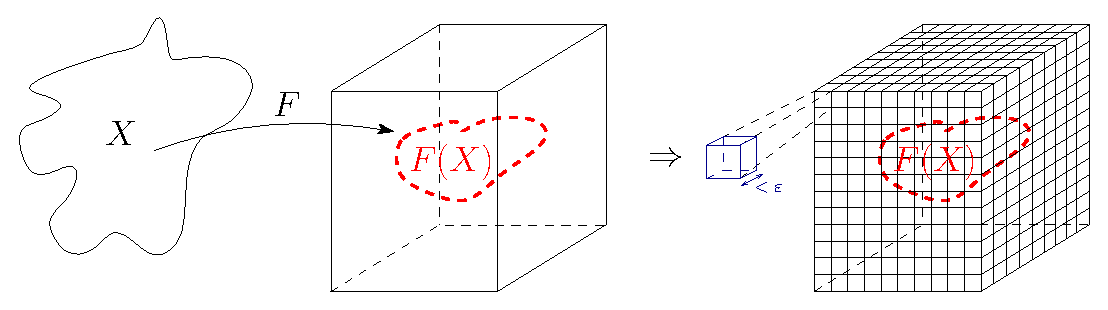
\includegraphics[width=0.85\textwidth]{MA3L11_1.eps}
		\label{MA3L11_1}
		\caption{Отображение $X$ в $\MR^n$ функцией $F$.}
		\label{fig:Покрытие	}
	\end{figure}
	Разрежем этот кубик на маленькие кубики диаметром меньше $\VE$ и берем те из них, которые задевают множество $F(X)$, причем берем эти кубики так, чтобы они попарно не пересекались, то есть грани распределяем между ними $\Rightarrow$ получаем $\MI_j$ - конечный набор попарно непересекающихся кубиков, диаметром меньше $\VE$, которые задевают образ $X$ при отображении $F$: $\MI_j \cap F(X) \neq \VN$. Тогда искомые множества:
	$$
		\forall j, \, X_j = F^{-1}(\MI_j)
	$$
	то есть это прообразы конечного набора попарно непересекающихся кубиков (а следовательно также представляют из себя набор попарно непересекающихся множеств, см. $2$ семестр, лекция $10$, упр. $1$).
	
	Проверим, что это искомые множества (для $3\VE$): возьмем произвольную $f \in K$ и произвольные $y,z \in X_j$, где $X_j$ - фиксированно. Все функции $f_1, \dotsc, f_m$ на прообразе этих кубов меняются мало (меньше, чем на $\VE$) по построению. Рассмотрим следующую разность: $|f(y) - f(z)|$, поскольку у нас была конечная $\VE$-сеть, то $\exists \, f_k \colon \sup\limits_{X_j}|f - f_k| < \VE$, то есть который мало отличается от $f$, тогда:  
	$$
		|f(y) - f(z)| = |f(y) - f_k(y) + f_k(y) - f(z)| \leq |f(y) - f_k(y)|  + |f_k(y) - f(z)| \leq
	$$
	$$
		\leq |f(y) - f_k(y)|  + |f_k(y) - f_k(z)| + |f_k(z) - f(z)| < 2\VE + |f_k(y) - f_k(z)|
	$$
	где последнее неравенство верно, поскольку $f_k$ принадлежит $\VE$-сети. Так как $y, z \in X_j$, то значения функции $f_k$ это $k$-ая координата при отображении в кубик $\MI_j$:
	$$
		F(X_j) = (f_1, \dotsc, f_k, \dotsc, f_M) \, (X_j) \subset \MI_j
	$$
	диаметр этого кубика меньше $\VE$, значит каждая координата отображения $F$ может изменяться не больше, чем на $\VE$ на нем, тогда:
	$$
		|f_k(y) - f_k(z)| < \VE \Rightarrow |f(y) - f(z)| < 3\VE
	$$
	
	($\Leftarrow$) Множество $K$ - замкнуто и ограниченно, следовательно необходимо построить $\VE$-сеть. Пусть мы разбили всё $X$ на $N$ частей: $$
		X = \bigsqcup\limits_{n = 1}^N X_n
	$$ 
	и на каждой из них функции из нашего семейства меняются мало. Поскольку это множество ограниченно, то все значения функций из $K$ лежат в некотором фиксированном отрезке $[-c,c]$. Разделим этот отрезок с шагом $\VE$ и в качестве $2\VE$-сети возьмем всевозможные следующие функции:
	$$
		 \forall j = \overline{1,N}, \, \forall x \in X_j, \, g \colon g(x) \equiv c_j
	$$
	число таких функций - конечное, поскольку у нас конечное число частей $X \Rightarrow$ это конечный набор. Таким образом, получили кусочно-постоянную функцию на $X$. Почему такой набор образует $2\VE$-сеть? Возьмем произвольную функцию $f$ и выберем $g$, которая нам потребуется так, чтобы было верно:
	$$
		|f(\omega) - g(\omega)| < 2\VE
	$$
	Пусть $\omega_j \in X_j \Rightarrow f(\omega_j) \in \, ]c_s, c_{s+1}[$ - какой-то промежуток. Пусть тогда $g(x) \equiv c_s$ на $X_j$, пройдемся так по всем $X_j \Rightarrow$ это кусочно-постоянная функция, тогда по условию $3)$:
	$$
		\forall \omega \in X_j, \, |f(\omega) - g(\omega)| = |f(\omega) - c_s| \leq |f(\omega) - f(\omega_j)| + |f(\omega_j) - c_s| < \VE + \VE = 2\VE
	$$
	Таким образом, мы построили $2\VE$-сеть и по критерию Хаусдорфа множество $K$ - компакт.
\end{proof}
\begin{rem}
	Для наглядности доказательства пункта ($\Rightarrow$), рассмотрим график одной функции $f(x)$, который лежит в интервале $[-1,1]$. Разделим область значений с шагом меньше $\VE$, возьмем промежутки попарно непересекающиеся (например, полуинтервалы) и обозначим их $\MI_j$. Если возьмем прообраз этого полуинтервала, то мы получим $X_j$:
	\begin{figure}[H]
		\centering
		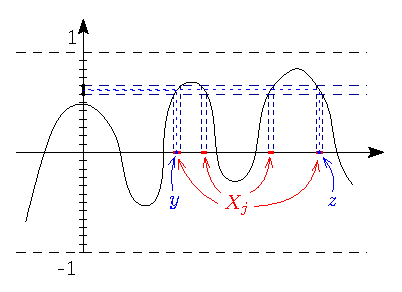
\includegraphics[width=0.45\textwidth]{MA3L11_2.eps}
		\label{MA3L11_1}
		\caption{Упрощение доказательства критерия компактности.}
		\label{fig:Покрытие	}
	\end{figure}
	Если мы возьмем какие-то две точки $y$ и $z$ в этом $X_j$, то значения в этих точках будут различаться меньше, чем на $\VE$: 
	$$
		\forall y,z \in X_j, \,	|f(y) - f(z)| < \VE
	$$ 
	Когда мы разобьем всю прямую на прообразы этих промежутков, то каждый из этих промежутков будет обладать таким свойством, что значения на них друг от друга отличаются меньше, чем на $\VE$. В теореме было сделано то же самое, но там была не одна функция, а $M$ штук.
\end{rem}
\begin{rem}
	Этот критерий компактности можно воспринимать, как критерий вполне ограниченности, если выкинуть из него замкнутость того множества, которое у нас есть.
\end{rem}
Следующая теорема по сути - есть следствие из только что доказанного критерия Компактности.

\begin{theorem}(\textbf{Арцела-Асколи})
	Множество $K \subset C[a,b]$ компактно $\Leftrightarrow$ 
	\begin{enumerate}[label={\arabic*)}]
		\item $K$ - замкнуто;
		\item $K$ - \uwave{равномерно ограниченно}, то есть: 
		$$	
			\exists \, C > 0 \colon \forall f \in K, \, \|f\| \leq C
		$$
		\item $K$ - \uwave{равностепенно непрерывно}, то есть: 
		$$
			\forall \VE > 0, \, \exists \, \delta > 0 \colon \forall f \in K, \, \forall x,y \in [a,b],\,  |x - y| < \delta \Rightarrow  |f(x) - f(y)| < \VE
		$$
	\end{enumerate}
\end{theorem}

\end{document}